\documentclass{article}
\usepackage[preprint, nonatbib]{neurips_2020}

\usepackage[utf8]{inputenc}
\usepackage[T1]{fontenc}
\usepackage{amsfonts}
\usepackage{microtype}
\usepackage{hyperref}

\usepackage{booktabs}
\usepackage{graphicx}
\usepackage[square,numbers]{natbib}
\usepackage{makecell}
\usepackage[ruled,vlined]{algorithm2e}
\usepackage{subcaption}
\usepackage{textcomp}

\title{Supplementary material for MeLES: Metric learning for event sequences with self-supervision}

\author{
Dmitrii Babaev\thanks{D. Babaev N. Ovsov and I. Kireev contributed equally to this work.} \\
% dmitri.babaev@gmail.com
Sberbank AI Lab
\And
Ivan Kireev \\
Sberbank AI Lab
\And
Nikita Ovsov \\
Sberbank AI Lab
\And
Nikita Ovsov \\
Sberbank AI Lab
\And
Maria Ivanova \\
Sberbank AI Lab
\And
Gleb Gusev \\
Sberbank AI Lab
\And
Alexander Tuzhilin \\
% \email{atuzhili@stern.nyu.edu}
New York University
}

\newcommand{\nt}[1]{{\bf [#1]}}

\begin{document}

\maketitle

\section{Experiments} \label{sec-exp}

\subsection{Baselines} \label{sec-baselines}

Here we describe the the details of producing hand-crafted features. All attributes of each transaction are either numerical (e. g. amount) or categorical (e.g. merchant type (mcc code), transaction type, etc.). 
For numerical type of attribute we apply aggregation functions, such as 'sum', 'mean', 'std', 'min', 'max', over all transactions per user. For example, if we apply 'sum' for the numerical field 'amount' we obtain a feature 'sum of all transaction amounts per user'. 
For categorical type of attribute we apply aggregation functions in a slightly different way. For each unique value of categorical attribute we apply aggregation functions, such as 'count', 'mean', 'std' over all transactions per user' numerical attribute. For example, if we apply 'mean' for the numerical attribute 'amount' grouped by categorical attribute 'mcc code' we obtain a feature 'mean amount of all transaction for each mcc code per user'. 
For example, for age prediction task we have one categorical attribute (small group) with 200 unique values, combining it with amount we can produce $200 * 3$ features ('group0 x amount x count',  'group1 x amount x count', ..., 'group199 x amount x count', 'group0 x amount x mean', ...). In total we use approx 605 features for age prediction task. For gender prediction task we have two categorical features: 'mcc code' with approx 200 unique values and 'tr type' with approx 100 unique values. So in total we use $200 * 3 + 100 * 3 + 5 = 905$ features.
Note, that hand-crafted features contain information about user spending profile but omit information about transactions temporal order.

\subsection{Embedding visualization}

In order to visualize MeLES embeddings in 2-dimensional space, we applied tSNE transformation~\cite{Maaten2008VisualizingDU} on them. tSNE transforms high-dimensional space to low-dimensional based on local relationships between points, so neighbour vectors in high-dimensional embedding space are pushed to be close in 2-dimensional space. We colorized 2-dimensional vectors using the target values of the datasets.

Note, that embeddings was learned in a fully self-supervised way from raw user transactions without any target information. Sequence of transactions represent user' behavior, thus the MeLES model captures behavioral patterns and outputs embeddings of users with similar patterns nearby.
As shown below, local clusters in embedding space correspond to distribution of user's attributes either age or gender.

tSNE vectors from the age prediction dataset are presented in the Figure \ref{fig-tsne-age}. We can observe 4 clusters: clusters for group '1' and '2' are on the opposite side of the cloud, clusters for groups '2' and '3' are in the middle.

Taking into account that age is an ordinal attribute, we can make an assumption about the ordering of age groups: $age(1) < age(3) < age(0) < age(2)$ or vice versa. ($age(bin)$ returns age of user for specific group).

tSNE points from gender prediction dataset are presented in the Figure \ref{fig-tsne-gender}. There are areas dominated by one gender label over another.

\begin{figure}
  \centering
  \caption{2D tSNE mapping of MeLES embeddings colored by target labels}
  \begin{subfigure}{0.5\textwidth}
    \caption{Age prediction dataset}
    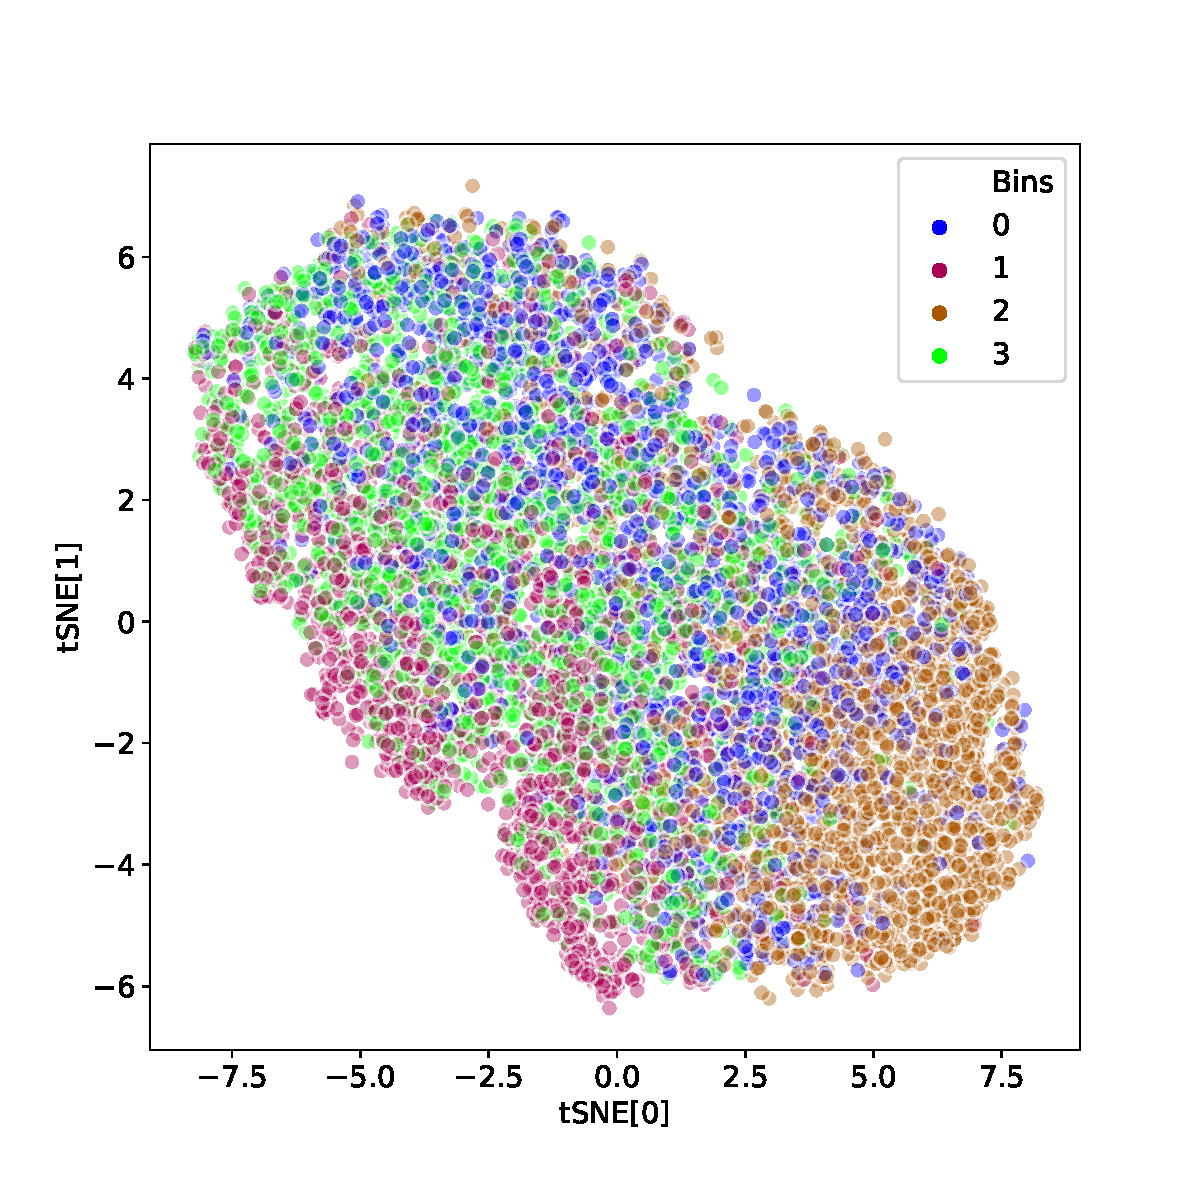
\includegraphics[width=\textwidth]{figures/age-pred-tsne.pdf}
    \label{fig-tsne-age}
  \end{subfigure}%
  \begin{subfigure}{0.5\textwidth}
    \caption{Gender prediction dataset}
    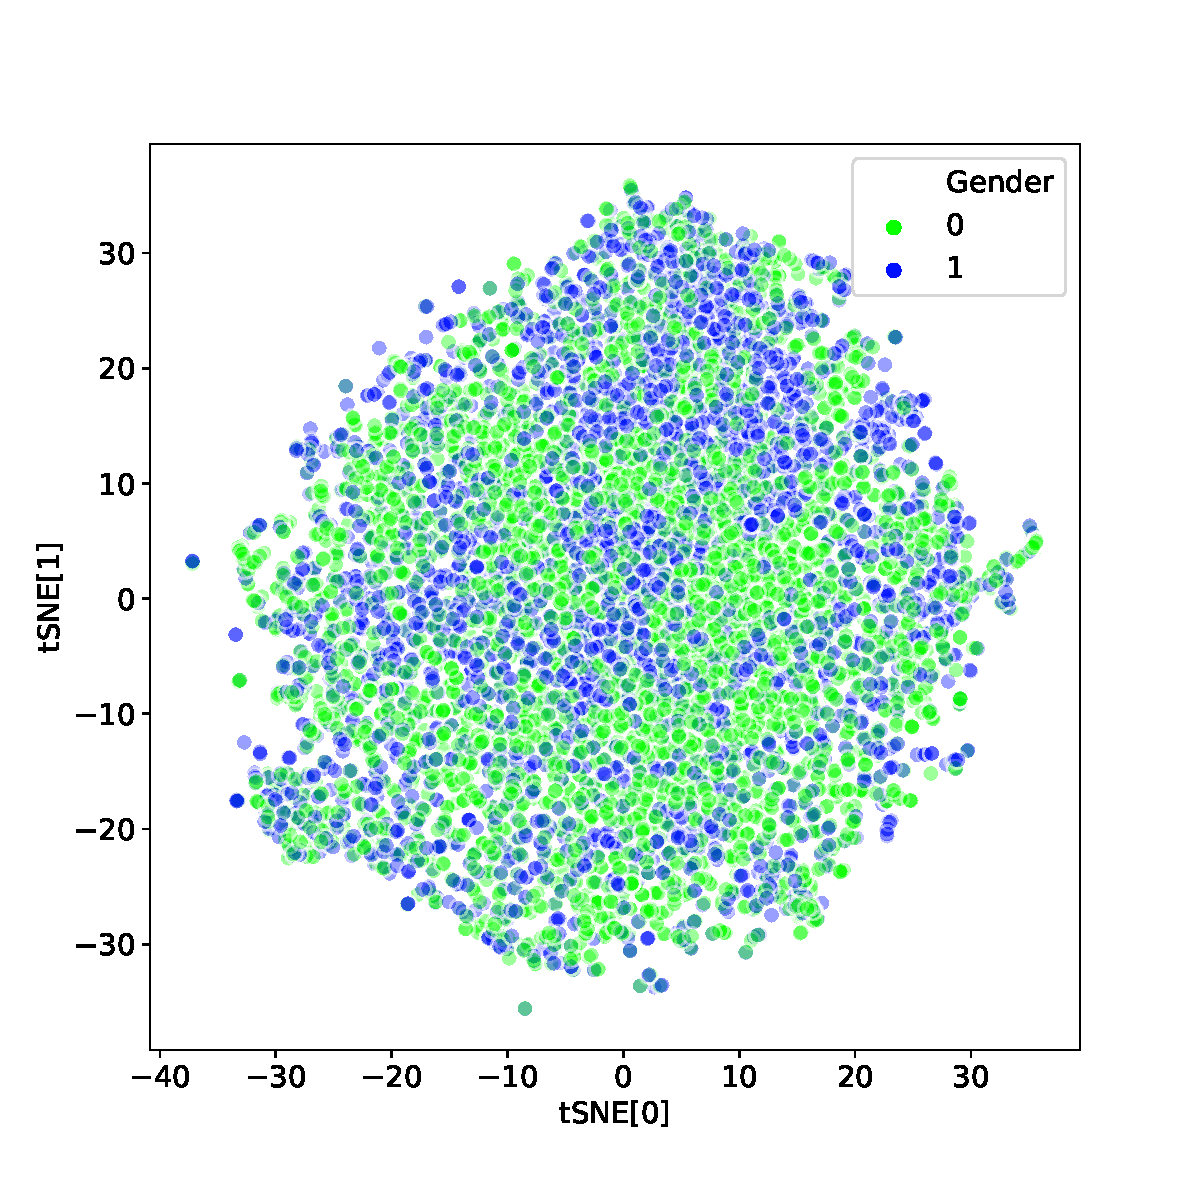
\includegraphics[width=\textwidth]{figures/gender-tsne.pdf}
    \label{fig-tsne-gender}
  \end{subfigure}
\end{figure}

\bibliographystyle{humannat}
\bibliography{neurips2020}

\end{document}